\documentclass[12pt,fleqn]{article}\usepackage{../../common}
\begin{document}
Yapay Zeka ile Problem Çözümü

Zeka nedir? Bu kavramın tanımı uzun süre filozofları, matematikçileri ve en
sonunda yazılım bilim adamlarını uğraştırdı.

Yapay Zeka olgusu, uzun bir değişim ve ne olduğunu tam bilmeyen bir
süreçten geçerek bu günlere geldi. En sonunda üzerinde mutabakat kurulan
tanım, yapay zekayı genel ve temel olarak iki kategoriye ayırdı.

Genel zeka altında, insanların bütün zihni güçlerini ve özelliklerini
birgün bilgisayar ile kopyalama, yapabilme çabası var. Tabii ki bu arayış
uzun bir zaman alacak.

Öteki dal temel zeka adı altında "sadece belli problemler için özel"
algoritmalar yaratarak, problem çözebilen bir zeka türü peşinde
koşmaktadır. Yani zeki bir vekil yaratıp onu problemin üzerine atmak, ya da
ufak bir temsilcimizi, bize benzeyen ufak bir kısmımızı yaratıp, onu
problem çözmek ile görevlendirmek diye nitelendirebileceğimiz bir zeka
türüdür aranan.

Teknik olarak detaya inersek, gerçek zamanda, sürekli girdi bilgisi
işleyerek hareket etmek zorunda olan zeka şeklini temel zeka altında
inceliyoruz. Karar verme olgusu bu vekil zeka için çok önemlidir, özellikle
belirsizlik altında bile karar verebilmek, vekil sistemler hayati önem
taşır.

Örnek Problem

Araştırmacılar, yapay zeka kodlarını denemek için bir deney ortamı ararken,
şunu düşündüler. Eğer hayat bir problemler dizisi, çözüm bekleyen sorunlar,
takip etmemiz gereken kurallar, ve plan gerektiren çözümler içeriyorsa, bu
ortamı benzetimlemenin en rahat yolu nedir?

Şans oyunları! Öyle ya, bir oyun hayatın ufak bir kopyası gibidir, kurallar
içerir, bir amaç vardır, plan gerektirir. Yapay zeka araştırmalarının oyun
oynamak üzerinde bu kadar durmasının sebebi budur.

8 Taş Oyunu

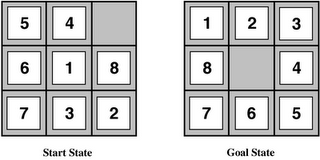
\includegraphics[height=4cm]{8-puzzle-start.png}

Yukarıdaki 8 taş oyununu, bilgisayara şöyle tanımlayabiliriz. Başlangıç
durumu olan taşları (solda) sonuç durumuna (sağa) dönüştürmek için gerekli
olan taş hareketleri bul ve raporla kullanıcıya bildir. Bilgisayar bu
sonuca birkac değişik algoritma takip ederek ulaşabilir.

Kör Arama

Kör, ya da mekanik, bir şekilde arama algoritmaları, başlangıç tahta durumu
üzerinde yapılabilecek bütün taş hareketlerini işletir ve sonuç tahtasını
kayıt eder. Mesela, başlangıç tahtasında 8 yukarı çıkabilir, 4 sağa
gidebilir. (Not: Kodlama açısından daha rahat olması için her taşın
hareketini değil, boşluğun hareketini baz almak daha rahat olur. Sonuç
aynı, ama kodlama daha rahat. Yani, boşluk sola gidebilir, aşagı
inebilir). Bu iki mümkün işlemden sonuç olarak iki yeni tahta
çıkacak. Onların da üzerinde olası bütün işlemleri yaparsak, daha da fazla
tahtalar çıkacak, vs. Bunu yaparken bir yandan sonuç tahtasına gelip
gelmediğimizi kontrol edersek, kör bir arama algoritması yazmış olacağız.

Bu işlemlerin sonuçlarını bir ağaç veri yapısı olarak temsil etmek uygun
olacak. Yani resimde görülen soldaki tahta üst düğüm, iki hareketten çıkan
olası yeni tahtalar o üst düğümün iki çocuğu olarak gösterilebilir. Böyle
giderek elimize bir ağaç yapısı çıkacak. Örneği aşağıda,

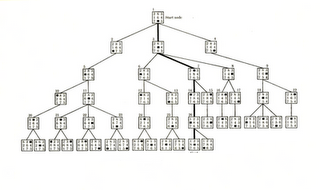
\includegraphics[height=8cm]{8-puzzle-tree.png}

Ağaç yapısı, birazdan göreceğimiz bütün arama algoritmalarının temelini
oluşturacak. Ama, bu ağacı yaratmanın değişik yolları var. Mesela, ağacın
her katını mı önce oluşturmak istersiniz, yoksa bir dalı sonuna kadar
derinliğine takip etmek, yoksa geri dönüp başka bir dalı mı tekrar
derinliğine aramak istersiniz.

LISP'e Giriş

Bu iki yolu, LİSP örnek kodu ile derinliğine inceleyelim. LİSP en eski
2. bilgisayar dilidir, ve Yapay Zeka araştırmaları için
yaratılmıştır. LİSP, fonksiyonları bile dinamik olarak yaratıp bildirgeç olarak
işlemlere verebilen bir dildir. Bu esnek yapısı yapay zeka
araştırmacılarının çok işine yaramıştır.

LISP dilinde temel veri yapısı "listedir". Mesela, yukarıdaki başlangıç
tahtasını LISP'de şöyle tanımlanabiliriz.

\begin{minted}[fontsize=\footnotesize]{python}
(setf tahta-baslangic '((5 4 nil)(6 1 8)(7 3 2)))
\end{minted}

Bu kullanımda dikkat ederseniz, bir listenin listesini tanımladık. Yani,
liste içeren bir liste. LISP referans kaynaklarından rahatça öğrenilebilir,
böylece LISP'in çoğu işleminin liste yapısı üzerinde tanımlanan işlemler
için olduğunu göreceksiniz. Zaten LISP'in ismi bile buradan gelir, LIST
Processing, türkçesi "liste işlemek".

Örnek diğer bazı liste işlemleri: (car liste) komutu listenin başındaki
değeri, (cdr liste) listenin geri kalan kısmını verir. (nth 2 liste)
listenin baştan 3. değerini getirir, (setf liste (append 'a liste)) liste
değişkenine 'a harfini ekler, vs..

Ağac yapısındaki her düğümün, arama algoritması için, üst düğümünü
hatırlaması gerekiyor. Ayrıca hangi taş kaydırma ile o tahta durumuna
geldiğini de hatırlaması gerekiyor. Çünkü sonuca geldiğimizde, oradan
tekrar başlangıca dönerek (üstü izleyerek) kaydırma işlemlerini ekrana
basarak göstereceğiz. Algoritmanın da amacı bu değil mi? Bilgisayarın
sonuca nasıl geldiğini bize göstermesi!

Bu sebeple, yeni büyütülmüş liste (listenin listesi) şu hale geldi. Örnek
olarak boşluğu aşağı kaydırarak, geldiğimiz bir tahtayı şöyle gösterelim.

\begin{minted}[fontsize=\footnotesize]{python}
;; listenin icine bakabilen islemler
(Defun Durum (dugum) (first dugum))
(Defun Kaydir (dugum) (second dugum))
(Defun Ust (dugum) (third dugum))

;; ornek bir tahta
(setq baslangic (((1 3 2)(5 4 6)(7 8 nil)) 
  'asagi (((1 3 2)(5 4 nil)(7 8 6))))

;; tahtayi ve islemleri kullanarak dugum hakkinda bazi raporlar
(print "kaydir islemi")
(kaydir baslangic)

(print "ust dugum")
(ust baslangic)

(print "tahta durumu")
(durum baslangic)
\end{minted}

"Üst" düğümün, çocuk düğümü içine nasıl konduğunu görüyoruz. Ağaçta daha
derine indikçe, liste içinde liste, onun içinde liste, onun da içinde liste
gibi bu yapı daha da derinleşecektir. C ya da Java gibi dillerinde imleç
(pointer) kullanarak aynı şey yapılabilir. Ama LISP bu ağaç yapısı için
bile liste kullanıyor. Merak etmeyin, imleç kullanımı kadar da etkili
oluyor.

Önce Genişliğine (Breadth-First) ve Önce Derinliğine (Depth-First) Arama

Ağaç yapısını tanımladıktan sonra, algoritmaya gelelim. Kat kat arama
algoritmasında, çocuk düğümleri yarattıktan sonra onları "işlenmek üzere
beklettiğimiz" bir listeye koyarız. (gene mi liste?) :)

Evet. Bu yapı üzerine ekleme yaparken, ya sonra, ya başa ekleme yapmak
mümkün. Eğer sona koyarsak, çocuklar en son girdiği yerden en son çıkacak,
eğer başa koyarsak girdiği gibi hemen çıkacaktır. Bu şekilde kullanımın
birincisi, listeyi kuyruk (queue) olarak, ikincisi yığıt (stack) olarak
kullanmak anlamına gelir. Yazılım bilimde bu iki olgu çok temeldir. Her
algoritma kitabında kuyruklar ve yığıtlar hakkında bilgi
alabilirsiniz. Sonuçta, çocukları yığıt üzerinde bekletmişsek, arama önce
genişliğine arama olur, kuyruk olarak bekletmişsek arama "önce derinliğine"
arama olur.

Bu iki arama şeklinin farkı niçin önemlidir? Burada esas sormamız gereken
şu olacak. Hangi arama şekli daha başarılıdır?

Bu sorunun cevabı algoritmik analiz ile verilebilir, fakat özet olarak
belirtmek gerekir ki, önce genişliğine aramak istatistiki olarak daha
başarılı oluyor. Derinliğine arama, ek başka algoritmalar ile destekli
olarak da başarılı olabiliyor.

Gereken Kodlar ve Programlar

Ekteki dosyalar LISP derleyicisi/yorumlayıcısi ve örnek kodlar
içeriyor. 

Önce genişliğine aramayı, derinliğine aramaya çevirmek için tek yapmanız
gereken yığıtı, kuyruğa çevirmektir.

Bir önceki yapay zeka yazısı, akıllı bilgisayarlar hakkında hayal kırıklığı
yaratmış olabilir. Sonuçta gösterdiğimiz algoritma, derinliğine ya da önce
genişliğine arasa bile, "bütün" sonuçları deniyor! Yani insan ile yarışmak
için aslında hafıza genişliğinden ve hesap hızından yararlanıyor. Peki
nerede zeka?

Bunu düşündüyseniz haklısınız. Hakikaten de, bu ilk bahsettiğimiz
algoritmalar "kaba-kuvvet algoritmaları" diye anılır. Direk ileri giderler,
ve gayet mekanik şekilde sonuca ulaşmaya uğraşırlar.

Fakat, bir insan olarak biliyoruz ki, akıllı olmanın bir özelliği de
öğrenmektir. Yani, bazı kısa yollar bulmak, bir takım dersler çıkartarak
sonuca daha hızlı ulaşmayı sağlamak insanların gayet doğal yaptığı
şeylerdir. Eğer bunlar kodlanmamışsa, oyun oynayan algoritmamız kaba
kuvvetten daha ileri gidemeyecek. Üstelik büyük problemler için o üstün
hızı bile yetişmeyebilir!

Pekala. Hadi o zaman şu programa biraz akıl verelim.

İzlenen Yolun Fiyatı

Algoritmamızın "arama" algoritmasını olarak isimlendirilmesinin sebebi,
mümkün olan birçok seçenek arasından kısa olanı bulmak için "arama"
yapmasıdır. Bilgisayarın önünde olan birçok seçeneğin her birinin fiyatı,
yani uzunluğu, birbirinden farklıdır. Akıllı bir programa lazım olan, bu
yollardan en kısa olanını bulmaktır. İnsanlar da, kendi düşüncelerini
hızlandırmak için birtakım yan algoritmalar geliştirirler ve çabuk sonuca
ulaşmaya uğraşırlar.

Bu fiyatı iki türlü ölçebiliriz. Birincisi, karar ağacında çözümü ararken o
an üzerinde bulunduğumuz düğüme gelmek için ödediğimiz fiyat (katedilen
yol), öteki de önümüzde katedeceğimiz geri kalan yoldur.

Katedilen yolun seçimde (arayışta) ne yararı var diye
düşünebilirsiniz. Eklemek gerekir ki, özellikle önce-derinliğine arama
algoritması bazen aynı düğüme değişik yollardan ulaşabiliyor. Bu gibi
durumlarda tuttuğumuz kayıtlarda aynı düğümü bulursak, ve bu düğümün
içerdiği yol daha pahalı ise, eskiyi listeden atıp, yerine yeni düğümü
koymamız gerekiyor.

Nihayet akıllı bir "seçim" yaptık.

Fakat hala geriye bakıyoruz. İleriye bakarak, bilgili bir tahminde hala
bulunmadık. İleriye dönük bir tahmin fonksiyonunu nasıl bilgisayarda kodlarız?
8'li Bulmaca oyununu düşünürsek; oyunun herhangi bir seviyesinde tahtaya
bakarak, en iyi yapılacak hareketi nasıl bulabiliriz?

Akıllı Tahmin

Öyle bir fonksiyon bulalım ki, elimizde olan düğümden yarattığımız çocuk
düğümler arasında hangisini takip edeceğimizi bize söylesin. Sözde program
şöyle olabilir.

\begin{itemize}
   \item Düğümü al
   \item Düğümün bütün olası çocuklarını yarat
   \item Her çocuk için, sonuç tahtasına olan tahmini bir uzaklık değeri
     hesapla
   \item Bu çocuk düğümler arasında sonuca en yakın olanı seç
\end{itemize}

Pekala, nedir bu uzaklık değeri? İşte akıl devreye burada giriyor.

Her tahta durumunun sonuca uzaklığı, tahmini olarak şöyle
hesaplanabilir. Mesela, başlangıçtaki her taşı, sonuç tahtasına bakarak
bulalım. Eğer sonuç tahtasındaki taş, başlangıçtaki aynı yerde değil ise,
ne kadar uzakta olduğunu bulalım.

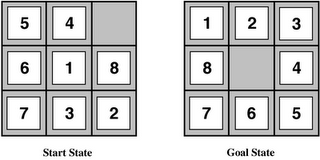
\includegraphics[height=4cm]{8-puzzle-start.png}

Üstteki iki tahta arasında, bu uzaklık değeri "5" taşı için "4"
olacaktır. Çünkü 1,1 eksen konumundan 3,3 konumuna gitmiştir. Ve aradaki
fark 2 aşağı 2 sağa gittiğimiz için 4'tür. Bu tür uzaklık hesabına
Manhattan uzaklığı deniyor, çünkü hepsi eşit bloklar arasında yürüyerek
giderken ölçülen türden bir hesap çeşididir.

Bu uzaklık hesabı, bir nevi şunu beyan etmektir - bu tahtayı, sonuç
tahtasına çevirmek için bu kadar hamle yapmak gerekiyor. Tabii ki bu hesap
kesin bir hesap değildir. Tam doğru da değildir, ama, olması da
gerekmez. Yeteri kadar doğru, ve en önemlisi, hiç bir zaman fazla keseden
atmayan bir hesap doğru seçim için yeterlidir. Çünkü, aynı şekilde "tam
doğru olmayan hesapları" öteki seçenekler için de yapıyoruz! Yani,
birbirine olan izafi bir doğruluk, sayının tamamen doğru olması etkisi
yapar.

LISP kodu

Ekteki kodlarda göreceğiniz gibi, LISP kodu için 2 tane fonksiyon tanımlamak
gerekti. G-güncel değişkeni 'geriye bakan' türden olan fiyatı-sabit-arama
algoritması için zaten gerekiyordu. Ekte olmayan, ama konu hakkında
görebileceğiniz bir algoritma sırf tahmine dayanarak seçim yapmaya uğraşır,
yani sadece t-guncel değerini kullanır. En güçlü olan yöntem, g-guncel ve
t-guncel'in 'toplamına' dayanarak seçim yapmaktır. Böylece hem o ana kadar
gözlediğimiz ölçümü, hem de ileriye bakarak yaptığımız tahmini aynı anda
gözönüne almıs oluyoruz.

İki hesabın birleşimine dayanarak seçim yapan arama algoritmasına A* (a
yıldız) algoritması denir. Bu kodu da a-yildiz-arama.lisp altında
bulabilirsiniz.

Ayrıca, ödev olarak (yapay zeka dersi için) bizim kodladığımız, A*'ı kendi
akıl fonksiyonu ile genişletip, kendi t-guncel kodunu yazmamız
gerekiyordu. 

Bu yeni A* t-guncel hesabı, hem taş uzaklığına dayanıyor, fakat bir toplam
daha ekliyor. Eğer iki taşı değiş tokuş yaptırmamız gerekiyorsa, bu normal
uzaklıktan çok daha pahalı bir işlemdir, ve 2 sayılması gerekir! Bu şekilde
yapılan toplamın, ve akabinde t-guncel değerinin, algoritmayı daha
geliştirdiğini göreceksiniz.

Yani biraz daha akıl kullanarak, işimizi kolaylaştırmış oluyoruz.

\inputminted[fontsize=\footnotesize]{python}{ortak.lisp}

\inputminted[fontsize=\footnotesize]{python}{kat-kat-ara.lisp}

\inputminted[fontsize=\footnotesize]{python}{kat-engelli-da.lisp}

\inputminted[fontsize=\footnotesize]{python}{iki-yonlu-arama.lisp}

\inputminted[fontsize=\footnotesize]{python}{git-gide-derin-kka.lisp}

\inputminted[fontsize=\footnotesize]{python}{fiyati-sabit-arama.lisp}

\inputminted[fontsize=\footnotesize]{python}{a-yildiz-arama.lisp}

Yapay Zeka ve Müsabaka

Bilgisayarlar bir problemi yapay zeka kullanarak çözerken, kullandıkları
teknikler; Karar ağacı, akıllı tahmin yeteneği ve o ana kadar geçilen yolu
hatırlamaktır.

Karar ağacı kullanırken, seçeceğimiz yolun doğru yol mu olup olmadığı
tahmin etmek için değerlendirme fonksiyonuna sorarız. Bu fonksiyon gerçek bir
tahmin mantığına ne kadar yakın ise, (yani uzman bir insana) arama da o
kadar başarılı olur.

Bu örnekten yola çıkarsak, karşılıklı müsabakalar da bir arama problemi
gibi görülebilir. Bir başlangıç noktası vardır, belli seçenekler vardır, bu
seçenekleri takip etmek için karar ağacı tekniği uygulanabilir.

Tek bir değişiklik ile: Artık kararların hepsi bize ait değil.

Altüst (Minimax) Algoritması

Mesela müsabaka, bir dama oyunu olsun. Oyun sırasında sıra bir bilgisayara,
bir karşı tarafa geçer. Bu yüzden iyi bir yapay zeka algoritması, hem kendi
hareketlerinin arasında "değerlendirme fonksiyonunun" en iyi bulduğunu seçmeli,
hem de, aynı zamanda rakibi için en kötü olacak yolu takip etmelidir.

Bu iki seçeneğe göre karar arama yapan algoritmaya altüst algoritması
diyoruz. Çünkü rakip için an alt değer ile, bilgisayar için en üst değeri
aynı anda arıyoruz.

Normal tek kişili arama algoritmalarında sadece "bir" ileriye bakarak
değerlendirme yapmış, ve en fazla olan seçeneği takip etmiştik. Altüst için
arama yaparken derinliğine ineceğiz, ve bu derinliği hafızamızın elverdiği kadar
yapabileceğiz. Çünkü, hamleye karşı hamle, ona karşı hamle derken en iyi
seçeneği bulabilmek için bazen oldukça derinlere inmek gerekebilir. 10 seviye
altta çok iyi gözüken bir birleşim olabilir, ama belki de 11. seviyede maçı
kaybediyoruz! Tabii dallanma seviyesi fazla olan oyunlarda (mesela satranç) bu
şekilde derinlik birçok bilgisayarı donanım olarak zorlayacaktır. Bu yüzden
Kasparov gibi bir ustayla ancak IBM'in satranç için özel yapılmış makinesi
rekabet edebiliyor.

Oyun: İtalyan Daması

Altüst algoritmasını dallanma faktörünün fazla olmadığı bir oyun üzerinde
göreceğiz. Bu oyunun ismi italyan daması. Bildiğimiz dama oyununa çok
benziyor, sadece taşlar düz olarak ileri, geri, sağa, sola gitmek yerine
çapraz hareket ediyorlar. Aynen damada olduğu gibi, en sona ulaşan taş kral
oluyor ve uzun sıçramalar yapabiliyor.

Ekte verilen LISP kodu üzerinde göreceğimiz gibi, programı temel
hareketler, değerlendirme fonksiyonu, algoritma ve ekrandan giriş yaparak
oynanabilen kısımlara ayırdık.

Altüst algoritması, özyineli olarak çalışan bir algoritmadır. Altüst, önce
derinliğine bir sekilde müsaade edildiği kadar (programcı tarafından)
derinliğe iner, ve vardığı en uç noktalardaki tahtaları değerlendirir. Geri
dönerken, bu değerlerden bazen "en az" olanı bazen "en fazla" olanı
seçer. En az/en fazla kıstası her seviyede bir değişir. Rakip hareketlerini
gösteren seviyede bulunuyorsak, enalt, kendi seviyemizde bulunuyorsak enüst
seçimi yaparız.

Üzerinde karşılaştırma yaptığımız sayı, değerlendirme fonksiyonunun tahta
hakkında biçtiği değerden başkası değildir. Bu tür değerlendirme fonksiyonlarını
A* algoritması altında görmüştük.

Tahta değerlerinin arasındaki seçimi özyineden geriye "dönerken"
yaptığımıza özellikle dikkat edin. Yani, 10. seviyeye indiysek ve bütün
önce-derinliğine olarak bir dalı açmış isek, ancak ondan sonra değerleri
birbirleri ile karşılaştırarak ve seçerek döndürmeye
başlıyoruz. Değerlendirme işleminin kendisi, derinliğin en sonundaki
tahtalar üzerinde yapılıyor. "Ara tahtaların" üzerinde değerlendirme
yapmıyoruz. (Bkz. \verb!tahta-degerlendir! fonksiyonu).

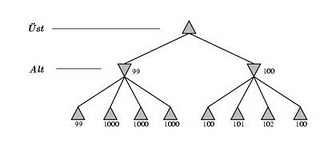
\includegraphics[height=4cm]{altust.jpg}

Örnekteki resimde 2. seviyeye 99 ve 100'ün dönmüş olduğunu
görüyoruz. 1. seviye de sırasıyla önce 99, sonra 100'ün dönmesi gerekir, ve
bunlardan 100 değeri 99'un üzerine çıkacaktır. Çünkü 1. seviye 'üst'
seviyesidir. Alt seviyesi olsa idi, 99 seçilecekti.

Ayrıca, seviyeye göre bazen alt, bazen üst değerler aradığımız için, hangi
seviyede olduğumuza bağlı olarak <> operatörlerini kullanmak yerine, hep aynı
operatörü (>) kullansak, ve karşılaştırma yaptığımız değeri sonraki seviyeye
aktarmadan önce eksi (-) ile çarpsak kod daha temiz olacak. Bunu ufak bir
algoritma numarası olarak görebilirsiniz. Değeri eksiye dönen bir değerin
üzerinde uygulanan büyüktür/küçüktür karşılaştırmalarının sonucu
otomatikman tersine döner (basit aritmetik). Eksiyi eksi ile çarpınca sayı
tekrar artıya döndüğü için özyineli olarak bu çarpımı tekrar tekrar
yapmamız mümkün olabiliyor. Ne güzel. Böylece iki tane if (ya da LISP cond)
ifadesi yazmaktan kurtulmuş olduk. Kod daha temiz hale geldi. Bahsedilen
çağırım şekli dama-alg.lisp dosyasındaki aşağıdaki satırda.

\begin{minted}[fontsize=\footnotesize]{python}
(setf dene (eniyi-hareket (tas-oynat 
   (first hareket-listesi) konumn)
(- derinlik 1)
(* onun-eniyi -1) ;; eksi carpimina dikkat
(* enyuksek-deger -1))) ;; ;; eksi carpimina dikkat
\end{minted}

Bir başka ilginç bir nokta da şudur: Rakibimizin tahtalarını ve kendi
tahtalarına değer biçerken hep aynı fonksiyonu kullanıyoruz. (Kod üzerinde
\verb!tahta-degeri(tahta)! LISP fonksiyonu). Bunun demektir ki Kendi oyun
bilgimize dayanarak rakibimizin ne yapacağını tahmin etmeye
uğraşıyoruz. Yani zihnen, sanal bir alemde "rakibimizin yerine" hamle
yapıyoruz ve bu sanal hamleye kendimize göre bir cevap veriyoruz. Hakikaten
de satranç, dama, kağıt oynarken yaptığımız da bu değil midir?

Eniyileştirme

Gördüğümüz gibi, altüst'ün temeli oldukça basit. Bundan sonrası, altüst'ü
hız ve hafıza bakımından eniyileştirme için yapılmıştır. Alfa-beta budaması
denen altüst uzantısı bu çerçevede düşünülmüştür.

Dama tahtaları arasında alt/üst irdelemesi yaparken, şunu düşünebiliriz:
Ağacın herhangi yerindeki oyuncunun varabileceği bir yer olarak bir n adlı
bir düğüm olduğunu düşünün; Eğer oyuncunun n'in bir üstü ya da daha
tepesinde (dallanma olarak) m adında daha iyi seçeneği var ise, n düğümü
oyun sırasında asla erişilmeyecektir. Bu yüzden n hakkında yeteri kadar
bilgiye sahip olduğumuzda (cocuklarından birkaçına bakarak), bu düğümü
tümden budayabiliriz.

Daha detaylı (ve matematiksel) bir örnekte göstermemiz gerekirse:

\begin{minted}[fontsize=\footnotesize]{python}
altust-degeri(en tepe) = 
   üst ( alt(3, 12, 8), alt(2, x, y), alt(14, 5, 2) )
altust-degeri(en tepe) = 
   üst ( 3, alt(2, x, y), 2)
altust-degeri(en tepe) = 
   üst ( 3, z, 2)
altust-degeri(en tepe) = 3
\end{minted}

Alt (2, x, y) fonksiyonunun değeri Z'ye eşitlendi (ve atıldı), x ve y'nin ne
olduğuna bile bakılmadan. Çünkü alt(2, x, y) dediğimiz zaman aynı anda şunu
söylemiş oluyoruz: "alt (2, x, y) en fazla 2 olabilir". Değil mi? Çünkü alt
fonksiyonunun gereği olarak zaten en aşağı olan değeri seçeceğiz. X ya da y
daha az olsa, onları seçerdik, daha fazla olsalar 2'yi seçeceğiz. Fakat,
elimizde KESİN bir 2 değeri "zaten" var ise, alt(2, x, y)'yi bir tarafa
atabiliriz, çünkü nasıl olsa alt(2, x, y)'nin sonucu 2'den daha iyi
olamazdı. DAHA İYİ'den kastımız üst fonksiyonu bakımından daha iyi demektir,
çünkü alt() fonksiyonlarının sonucu üst() fonksiyonuna gidiyor, biliyorsunuz.

Sonuçta, soyut olarak düşünerek alt(2, x, y)'nin üzerinde 2 yönlü bir
traşlama yapıyoruz denebilir. X ve Y'nin 2'den fazla olmasını fonksiyonun
kendisi traşlıyor. Daha az olabilme ihtimallerini'de, elimizde zaten olan 2
değeri traşlıyor, çünkü bu iki değerinin ne yaparsak yapalım üstüne
çıkamayacağız. Alt değerleri, üstte toplandığı için...

Alfa beta budaması ismini ağaçta gezinirken o ana kadar en üst bulunmuş
olan değeri alfa değişkeninde, ve en alt bulunmuş değeri beta değişkeninde
sürekli olarak yanında gezdirmesinden alır. En alt ve en üst değerler
aranırken sürekli alfa ve beta'ya karşılaştırma yapılır. Alfa/beta
penceresinin içine düşmeyen seçenekler ve onların alt-ağaçları tamamen
budanır. Bu şekilde yer ve zamandan oldukça istifade etmemiz mümkündür.

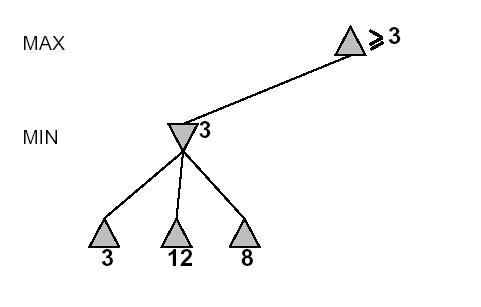
\includegraphics[height=4cm]{altust_budama_1.jpg}

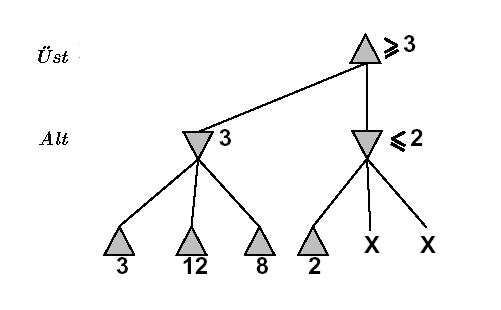
\includegraphics[height=4cm]{altust_budama_2.jpg}

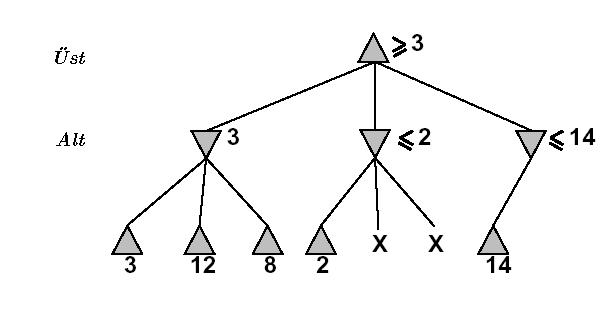
\includegraphics[height=4cm]{altust_budama_3.jpg}

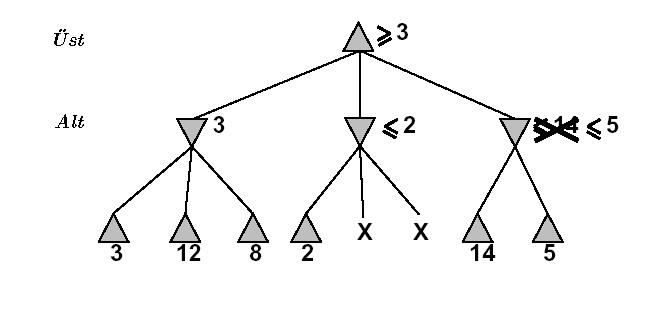
\includegraphics[height=4cm]{altust_budama_4.jpg}

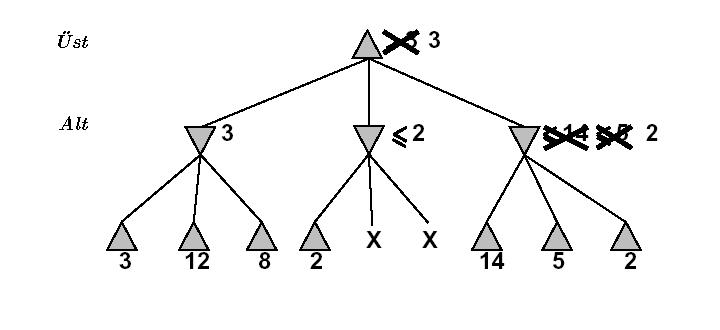
\includegraphics[height=4cm]{altust_budama_5.jpg}

\inputminted[fontsize=\footnotesize]{python}{dama-alg.lisp}

\inputminted[fontsize=\footnotesize]{python}{dama-deger.lisp}

\inputminted[fontsize=\footnotesize]{python}{dama-oyna.lisp}

\inputminted[fontsize=\footnotesize]{python}{dama-temel.lisp}

\inputminted[fontsize=\footnotesize]{python}{dama-test.lisp}

Tek hamlelik bir oyun oynayalım, ve bilgisayarın karşılığını görelim, 

\begin{minted}[fontsize=\footnotesize]{python}
!clisp dama-test.lisp
\end{minted}

\begin{verbatim}

"Tamam. Temel Birim Testler Gecti" 
"Tamam. Algoritma Birim Testleri Gecti" 
WARNING: DEFUN/DEFMACRO: redefining function TAHTA-DEGERI in
         /home/burak/Documents/classnotes/app-math-tr/probsolve/dama-deger.lisp,
         was defined in
         /home/burak/Documents/classnotes/app-math-tr/probsolve/dama-alg.lisp
"Tamam. Degerlendirme Birim Testleri Gecti" 
+=0===1===2===3===4===5===6===7-+
7   | b |   | b |   | b |   | b |
|===============================|
6 b |   | b |   | b |   | b |   |
|===============================|
5   | b |   | b |   | b |   | b |
|===============================|
4   |   |   |   |   |   |   |   |
|===============================|
3   |   |   |   |   |   |   |   |
|===============================|
2 s |   | s |   | s |   | s |   |
|===============================|
1   | s |   | s |   | s |   | s |
|===============================|
0 s |   | s |   | s |   | s |   |
+=0===1===2===3===4===5===6===7=+

"su hareketi yaptiniz" 
((0 2) (1 3)) 
+=0===1===2===3===4===5===6===7-+
7   | b |   | b |   | b |   | b |
|===============================|
6 b |   | b |   | b |   | b |   |
|===============================|
5   | b |   | b |   | b |   | b |
|===============================|
4   |   |   |   |   |   |   |   |
|===============================|
3   | s |   |   |   |   |   |   |
|===============================|
2   |   | s |   | s |   | s |   |
|===============================|
1   | s |   | s |   | s |   | s |
|===============================|
0 s |   | s |   | s |   | s |   |
+=0===1===2===3===4===5===6===7=+

"bilgisayarin hareketi" 
((1 5) (0 4)) 
+=0===1===2===3===4===5===6===7-+
7   | b |   | b |   | b |   | b |
|===============================|
6 b |   | b |   | b |   | b |   |
|===============================|
5   |   |   | b |   | b |   | b |
|===============================|
4 b |   |   |   |   |   |   |   |
|===============================|
3   | s |   |   |   |   |   |   |
|===============================|
2   |   | s |   | s |   | s |   |
|===============================|
1   | s |   | s |   | s |   | s |
|===============================|
0 s |   | s |   | s |   | s |   |
+=0===1===2===3===4===5===6===7=+
\end{verbatim}

Biz siyah (s) tarafıyız ve ilk hamleyi \verb!0,2! kordinatından \verb!1,3!
kordinatına dogru yaptık. Bilgisayar buna karşılık \verb!1,5!'ten
\verb!0,4!'e doğru bir hamle yapti. %

\end{document}
